\def\topic{Recursion}
\input{comp125lectureHeader}

\begin{figure}
\centering	
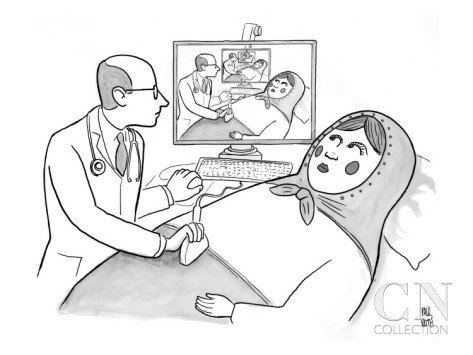
\includegraphics[width=.4\textwidth]{images/russiandoll.jpg}
\caption{Source: \href{https://condenaststore.com/featured/a-doctor-is-seen-giving-an-sonogram-to-a-russian-paul-noth.html}{Credit: Paul Noth}}
\end{figure}

\section{Background}

Before we jump into the concept of recursive solutions and definition of recursive methods, it's critical that we understand how method calls work.

We will use the following example to explain method calls:

\begin{lstlisting}
public class Client {
	public static void caller() {
		int a = 10, b = 5;
		boolean flag = callee(a+3, b*2);
	}
	
	public static boolean callee(int m, int n) {
		boolean result;
		if(m%2 == n%2) {
			result = true;
		}
		else {
			result = false;
		}
		return result;
	}
}
\end{lstlisting}

\begin{enumerate}
  \item Any piece of code that we write is inside some method (besides declaring variables).
  \item When a piece of code inside one method (\texttt{caller}) calls another method (\texttt{callee}), the following things occurs,
  \begin{enumerate}
  \item The control transfers from \texttt{caller} to \texttt{callee}. 
  \item Actual parameters (\texttt{a+3, b*2} = \texttt{13,10}) passed are copied into the formal parameters (\texttt{m,n}). 
  \item An entry for \texttt{callee} with associated formal parameters and local variables is added on top of the \texttt{call stack}.
  \end{enumerate}
  \bgroup \tikzset{png export} \begin{tikzpicture}
\scopeblock{functionName=caller(),variables={{"a=10", "b=5", "flag"}},width=3.2}
\scopeblock{x=5,functionName={callee(a+3, b*2)},variables={{"m=13","n=10","result=0"}},width=3.2}
\arrow{startX=3,startY=2.3,endX=4.8,endY=2.3}
\draw[rounded corners,fill=red!10!white] (9,0) rectangle (16,0.5) node[pos=.5] {caller()};
\draw[rounded corners,fill=green!10!white] (9.5,0.5) rectangle (15.5,1) node[pos=.5] {callee(13, 10)};
\end{tikzpicture} \egroup

  \item The method \texttt{callee(13, 10)} terminates with a \texttt{return} statement (or when the last statement  executes). The following happen when \texttt{callee} terminates,
  \begin{enumerate}
  \item The value returned (in case of non-void methods) replaces the method call. Thus \texttt{flag} inside \texttt{caller} becomes \texttt{false}.
  \item The entry for \texttt{callee} is removed from the call stack. All formal parameters and local variables are destroyed.
  \end{enumerate}
  \bgroup \tikzset{png export} \begin{tikzpicture}
	\scopeblock{functionName=caller(),variables={{"a=10", "b=5", "flag=false"}},width=3.2}
	\scopeblock{x=5,functionName={callee(a+3, b*2)},variables={{"m=13","n=10","result=0"}},width=3.2}
	\arrow{startX=4.8,startY=2.3,endX=2.5,endY=0.3,style=dashed,label=false}
	\draw[rounded corners,fill=green!10!white] (9,0) rectangle (16,0.5) node[pos=.5] {caller()};
	\draw[red, very thick](5,2.5) -- (8,0);
	\draw[red, very thick](5,0) -- (8,2.5);
  \end{tikzpicture} \egroup
\end{enumerate}

\section{Overview}
Recursion is the process of \emph{reducing a problem into a simpler form of itself}.

For example, $x^n$ (read as \emph{$x$ to the power of $n$}) is defined as $x * x * \cdots n$ times.

\large
\begin{align*}
x^n&=x * x * x \cdots n \text{times}\\
       &=[x * x * x \cdots (n-1) \text{times}] * x\\
       &=x^{n-1} * x
\end{align*} 
\normalsize


If we were writing a method to compute $x^n$, how would we define it?

It needs the values for $x$ and $n$, and returns the result ($x^n$).

So something like:

\begin{lstlisting}
public static double power(double x, int n)
\end{lstlisting}

Now, the formula tells us that this method, when called with parameters $x$ and $n$, should return $x^{n-1} * x$. So,

\begin{lstlisting}
public static double power(double x, int n) {
	return power(x, n-1) * x;
}
\end{lstlisting}

But if we do this, our method calls (while computing $2^3$) will look like,

\begin{itemize}
\item power(2, 3) $\rightarrow$
\item power(2, 2) $\rightarrow$
\item power(2, 1) $\rightarrow$
\item power(2, 0) $\rightarrow$
\item power(2, -1) $\rightarrow$
\item $\cdots$ forever
\end{itemize}

\newpage

Which means, at some stage we need to stop the method calls.

What do we know about the power operation? 

\begin{center}
\huge{$x^0$ = 1}
\end{center}
\normalsize

If we reach $n=0$, we can return 1.
This is called the termination step.

Our final method:

\begin{lstlisting}
public static double power(double x, int n) {
	if(n == 0) {
		return 1;
	}
	else {
		return power(x, n-1) * x;
	}
}
\end{lstlisting}

\section{Detailed example}

\begin{lstlisting}
public class Client {
	public static void main(String[] args) {
		int a = 4;
		int b = sum(a);
	}
	
	public static int sum(int n) {
		if(n == 0) {
			return 0;
		}
		int result = n + sum(n-1);
		return result;
	}
}
\end{lstlisting}

\newpage

\bgroup \tikzset{png export} \begin{tikzpicture}
\scopeblock{functionName=main,variables={{"a=4","b=sum(4)"}},width=3.2}	
\draw[rounded corners,fill=green!10!white] (9,0) rectangle (16,0.5) node[pos=.5] {main};
\end{tikzpicture} \egroup
\vskip0.6cm

\bgroup \tikzset{png export} \begin{tikzpicture}
\scopeblock{functionName=main,variables={{"a=4","b=sum(4)"}},width=3.2}	
\scopeblock{x=5,functionName=sum(4),variables={{"n=4","result= 4 + sum(3)"}},width=3.2}
\arrow{startX=3,startY=2.3,endX=5.2,endY=2.3}
\draw[rounded corners,fill=red!10!white] (9,0) rectangle (16,0.5) node[pos=.5] {main};
\draw[rounded corners,fill=green!10!white] (9.5,0.5) rectangle (15.5,1) node[pos=.5] {sum(4)};
\end{tikzpicture} \egroup

\vskip0.6cm

\bgroup \tikzset{png export} \begin{tikzpicture}
\scopeblock{functionName=sum(4),variables={{"n=4","result= 4 + sum(3)"}},width=3.2}
\scopeblock{x=5,functionName=sum(3),variables={{"n=3","result= 3 + sum(2)"}},width=3.2}
\arrow{startX=3,startY=2.3,endX=5.2,endY=2.3}
\draw[rounded corners,fill=red!10!white] (9,0) rectangle (16,0.5) node[pos=.5] {main};
\draw[rounded corners,fill=red!10!white] (9.5,0.5) rectangle (15.5,1) node[pos=.5] {sum(4)};
\draw[rounded corners,fill=green!10!white] (10,1) rectangle (15,1.5) node[pos=.5] {sum(3)};
\end{tikzpicture} \egroup

\vskip0.6cm

\bgroup \tikzset{png export} \begin{tikzpicture}
\scopeblock{functionName=sum(3),variables={{"n=3","result= 3 + sum(2)"}},width=3.2}
\scopeblock{x=5,functionName=sum(2),variables={{"n=2","result= 2 + sum(1)"}},width=3.2}
\arrow{startX=3,startY=2.3,endX=5.2,endY=2.3}
\draw[rounded corners,fill=red!10!white] (9,0) rectangle (16,0.5) node[pos=.5] {main};
\draw[rounded corners,fill=red!10!white] (9.5,0.5) rectangle (15.5,1) node[pos=.5] {sum(4)};
\draw[rounded corners,fill=red!10!white] (10,1) rectangle (15,1.5) node[pos=.5] {sum(3)};
\draw[rounded corners,fill=green!10!white] (10.5,1.5) rectangle (14.5,2) node[pos=.5] {sum(2)};
\end{tikzpicture} \egroup

\vskip0.6cm

\bgroup \tikzset{png export} \begin{tikzpicture}
\scopeblock{functionName=sum(2),variables={{"n=2","result= 2 + sum(1)"}},width=3.2}
\scopeblock{x=5,functionName=sum(1),variables={{"n=1","result= 1 + sum(0)"}},width=3.2}
\arrow{startX=3,startY=2.3,endX=5.2,endY=2.3}
\draw[rounded corners,fill=red!10!white] (9,0) rectangle (16,0.5) node[pos=.5] {main};
\draw[rounded corners,fill=red!10!white] (9.5,0.5) rectangle (15.5,1) node[pos=.5] {sum(4)};
\draw[rounded corners,fill=red!10!white] (10,1) rectangle (15,1.5) node[pos=.5] {sum(3)};
\draw[rounded corners,fill=red!10!white] (10.5,1.5) rectangle (14.5,2) node[pos=.5] {sum(2)};
\draw[rounded corners,fill=green!10!white] (11,2) rectangle (14,2.5) node[pos=.5] {sum(1)};
\end{tikzpicture} \egroup

\vskip0.6cm

\bgroup \tikzset{png export} \begin{tikzpicture}
\scopeblock{functionName=sum(1),variables={{"n=1","result= 1 + sum(0)"}},width=3.2}
\scopeblock{x=5,functionName=sum(0),variables={{"n=0","result= 0"}},width=3.2}
\arrow{startX=3,startY=2.3,endX=5.2,endY=2.3}
\draw[rounded corners,fill=red!10!white] (9,0) rectangle (16,0.5) node[pos=.5] {main};
\draw[rounded corners,fill=red!10!white] (9.5,0.5) rectangle (15.5,1) node[pos=.5] {sum(4)};
\draw[rounded corners,fill=red!10!white] (10,1) rectangle (15,1.5) node[pos=.5] {sum(3)};
\draw[rounded corners,fill=red!10!white] (10.5,1.5) rectangle (14.5,2) node[pos=.5] {sum(2)};
\draw[rounded corners,fill=red!10!white] (11,2) rectangle (14,2.5) node[pos=.5] {sum(1)};
\draw[rounded corners,fill=green!10!white] (11.5,2.5) rectangle (13.5,3) node[pos=.5] {sum(0)};
\end{tikzpicture} \egroup

\vskip0.6cm

\bgroup \tikzset{png export} \begin{tikzpicture}
\scopeblock{functionName=sum(1),variables={{"n=1","result= 1 + sum(0)"}},width=3.2}
\scopeblock{x=5,functionName=sum(0),variables={{"n=0","result= 0"}},width=3.2}
\arrow{style=dashed,startX=5.2,startY=2.3,endX=2.8,endY=0.8,label=0}
\draw[red, very thick](5,2.5) -- (8,0);
\draw[red, very thick](5,0) -- (8,2.5);
\draw[rounded corners,fill=red!10!white] (9,0) rectangle (16,0.5) node[pos=.5] {main};
\draw[rounded corners,fill=red!10!white] (9.5,0.5) rectangle (15.5,1) node[pos=.5] {sum(4)};
\draw[rounded corners,fill=red!10!white] (10,1) rectangle (15,1.5) node[pos=.5] {sum(3)};
\draw[rounded corners,fill=red!10!white] (10.5,1.5) rectangle (14.5,2) node[pos=.5] {sum(2)};
\draw[rounded corners,fill=green!10!white] (11,2) rectangle (14,2.5) node[pos=.5] {sum(1)};
\end{tikzpicture} \egroup

\vskip0.6cm

\bgroup \tikzset{png export} \begin{tikzpicture}
\scopeblock{functionName=sum(2),variables={{"n=2","result= 2 + sum(1)"}},width=3.2}
\scopeblock{x=5,functionName=sum(1),variables={{"n=1","result=1"}},width=3.2}
\arrow{style=dashed,startX=5.2,startY=2.3,endX=2.8,endY=0.8,label=1}
\draw[red, very thick](5,2.5) -- (8,0);
\draw[red, very thick](5,0) -- (8,2.5);
\draw[rounded corners,fill=red!10!white] (9,0) rectangle (16,0.5) node[pos=.5] {main};
\draw[rounded corners,fill=red!10!white] (9.5,0.5) rectangle (15.5,1) node[pos=.5] {sum(4)};
\draw[rounded corners,fill=red!10!white] (10,1) rectangle (15,1.5) node[pos=.5] {sum(3)};
\draw[rounded corners,fill=green!10!white] (10.5,1.5) rectangle (14.5,2) node[pos=.5] {sum(2)};
\end{tikzpicture} \egroup

\vskip0.6cm

\bgroup \tikzset{png export} \begin{tikzpicture}
\scopeblock{functionName=sum(3),variables={{"n=3","result= 3 + sum(2)"}},width=3.2}
\scopeblock{x=5,functionName=sum(2),variables={{"n=2","result=3"}},width=3.2}
\arrow{style=dashed,startX=5.2,startY=2.3,endX=2.8,endY=0.8,label=3}
\draw[red, very thick](5,2.5) -- (8,0);
\draw[red, very thick](5,0) -- (8,2.5);
\draw[rounded corners,fill=red!10!white] (9,0) rectangle (16,0.5) node[pos=.5] {main};
\draw[rounded corners,fill=red!10!white] (9.5,0.5) rectangle (15.5,1) node[pos=.5] {sum(4)};
\draw[rounded corners,fill=green!10!white] (10,1) rectangle (15,1.5) node[pos=.5] {sum(3)};
\end{tikzpicture} \egroup

\vskip0.6cm

\bgroup \tikzset{png export} \begin{tikzpicture}
\scopeblock{functionName=sum(4),variables={{"n=4","result= 4 + sum(3)"}},width=3.2}
\scopeblock{x=5,functionName=sum(3),variables={{"n=3","result=6"}},width=3.2}
\arrow{style=dashed,startX=5.2,startY=2.3,endX=2.8,endY=0.8,label=6}
\draw[red, very thick](5,2.5) -- (8,0);
\draw[red, very thick](5,0) -- (8,2.5);
\draw[rounded corners,fill=red!10!white] (9,0) rectangle (16,0.5) node[pos=.5] {main};
\draw[rounded corners,fill=green!10!white] (9.5,0.5) rectangle (15.5,1) node[pos=.5] {sum(4)};
\end{tikzpicture} \egroup

\vskip0.6cm

\bgroup \tikzset{png export} \begin{tikzpicture}
\scopeblock{functionName=main,variables={{"a=4","b = sum(4)"}},width=3.2}	
\scopeblock{x=5,functionName=sum(4),variables={{"n=4","result=10"}},width=3.2}
\arrow{style=dashed,startX=5.2,startY=2.3,endX=2.8,endY=0.8,label=10}
\draw[red, very thick](5,2.5) -- (8,0);
\draw[red, very thick](5,0) -- (8,2.5);
\draw[rounded corners,fill=green!10!white] (9,0) rectangle (16,0.5) node[pos=.5] {main};
\end{tikzpicture} \egroup

\vskip0.6cm

\bgroup \tikzset{png export} \begin{tikzpicture}
\scopeblock{functionName=main,variables={{"a=4","b=10"}},width=3.2}	
\draw[red, very thick](0,2.5) -- (3,0);
\draw[red, very thick](0,0) -- (3,2.5);
\end{tikzpicture} \egroup

\newpage
\section{Tracing some more recursive code}

\begin{exercise}[6]
Trace the call to recursive method \texttt{foo}

\begin{lstlisting}
public class Client {
	public static void main(String[] args) {
		int a = 8327;
		int b = foo(a);
	}
	
	public static int foo(int n) {
		if(n==0) {
			return 0;
		}
		int result = n%10 + sum(n/10);
		return result;
	}
}
\end{lstlisting}
\end{exercise}
\begin{answer}
\begin{verbatim}
foo(8327) = 7 + foo(832)
foo(832) = 2 + foo(83)
foo(83) = 3 + foo(8)
foo(8) = 8 + foo(0)
foo(0) = 0
Therefore,
foo(8) = 8 + 0 = 8
foo(83) = 3 + 8 = 11
foo(832) = 2 + 11 = 13
foo(8327) = 7 + 13 = 20
b = 20	
\end{verbatim}
\end{answer}

\newpage

\begin{exercise}[6]
Trace the call to recursive method \texttt{foo}

\begin{lstlisting}
public class Client {
	public static void main(String[] args) {
		int a = 42, b = 140;
		int c = foo(a, b);
	}
	
	public static int foo(int n) {
		if(b==0) {
			return a;
		}
		int result = foo(b, a%b);
		return result;
	}
}
\end{lstlisting}
\end{exercise}
\begin{answer}
\begin{verbatim}
foo(42, 140) = foo(140, 42)
foo(140, 42) = foo(42, 14)
foo(42, 14) = foo(14, 0)
foo(14, 0) = 14
Therefore,
foo(42, 14) = 14
foo(140, 42) = 14
foo(42, 140) = 14
c = 14
\end{verbatim}
\end{answer}

\section{Recursion with Strings}

Recursive solutions can be very useful when working with Strings.

For example, if you want to reverse a String, you can reverse all but the first character and then append the first character at the end of that.

\begin{lstlisting}
public static String reverse(String s) {
	if(s.length() < 2) {
		return s;
	}
	char first = s.charAt(0);
	String rest = s.substring(1);
	return reverse(rest) + first;
}
\end{lstlisting}

Once you have the method \texttt{reverse}, checking if a String is a palindrome (same when reversed) or not is a breeze.

\begin{lstlisting}
public static boolean isPalindrome(String s) {
	if(s.length() < 2) {
		return true;
	}
	return s.equals(reverse(s));
}
\end{lstlisting}
\section{Actually useful recursion}

The examples that we saw so far are pedagogical in nature, that is, they are easy to understand. However, they are not very useful in real life as the same thing can be done without using recursion (using an \textit{iterative} solution).

However, recursion \textbf{is} very powerful as explained in the following problem and its (recursive) solution.


\subsection{The Problem}

Given an integer array (\texttt{arr}) and another integer (\texttt{target}), finding out whether some items of \texttt{arr} add up to \texttt{target} or not.

\begin{itemize}
  \item For every item in the array (\texttt{arr[i])}, either the item is a part of the subset that adds up to the target, or its not.
  \item If that item \textbf{is} a part of the subset adding up to the \texttt{target}, we need to check if the rest of the array adds up to \texttt{target - arr[i]}
  \item If that item is \textbf{not} a part of the subset adding up to the \texttt{target}, we need to check if the rest of the array adds up to \texttt{target}
  \item But how do we tell the method that we want to look through \textbf{the rest of the} array? By passing a starting index.
  \item If that index reaches \texttt{arr.length} and we haven't successfully \textit{constructed} \texttt{target}, we can return \texttt{false}
\end{itemize}

\newpage

\begin{lstlisting}
public static boolean addUpTo(int[] arr, int target, int start) {
	if(target == 0) {
		return true;
	}
	
	if(start == arr.length) {
		return false;
	}
	//can target can be constructed with arr[start]?
	if(addUpTo(arr, target - arr[start], start + 1)) {
		return true;
	}
	//can target can be constructed without arr[start]?
	if(addUpTo(arr, target, start + 1)) {
		return true;
	}
	return false;
}
\end{lstlisting}

The beauty about the method is that all the current method call needs to do is explore two options, 

\begin{itemize}
  \item to use the current item, or,
  \item not (to use the current item)
\end{itemize}

and the the delegate method call will worry about the rest.
\input{comp125lectureFooter}
